Este capítulo apresentará o método proposto por este trabalho para o projeto de uma prótese ativa baseada em sensores e aprendizado de máquina.

\section{\todo{Corrigir este título}O sistema embarcado da prótese}
\label{sec:metodo_protese}

O projeto desenvolvido neste trabalho é uma prótese robótica para membros inferiores ou, mais especificamente, para a articulação do tornozelo. Esta prótese será construída a partir de modelos de próteses para impressoras 3D, aproveitando-se as partes mecânicas. A intenção é manter um baixo custo de produção. O sistema é projetado para funcionar em uma prótese transtibial.

\begin{figure}[h]
	\caption{\label{fig:big_picture}Visão geral do protótipo}
	\begin{center}
	    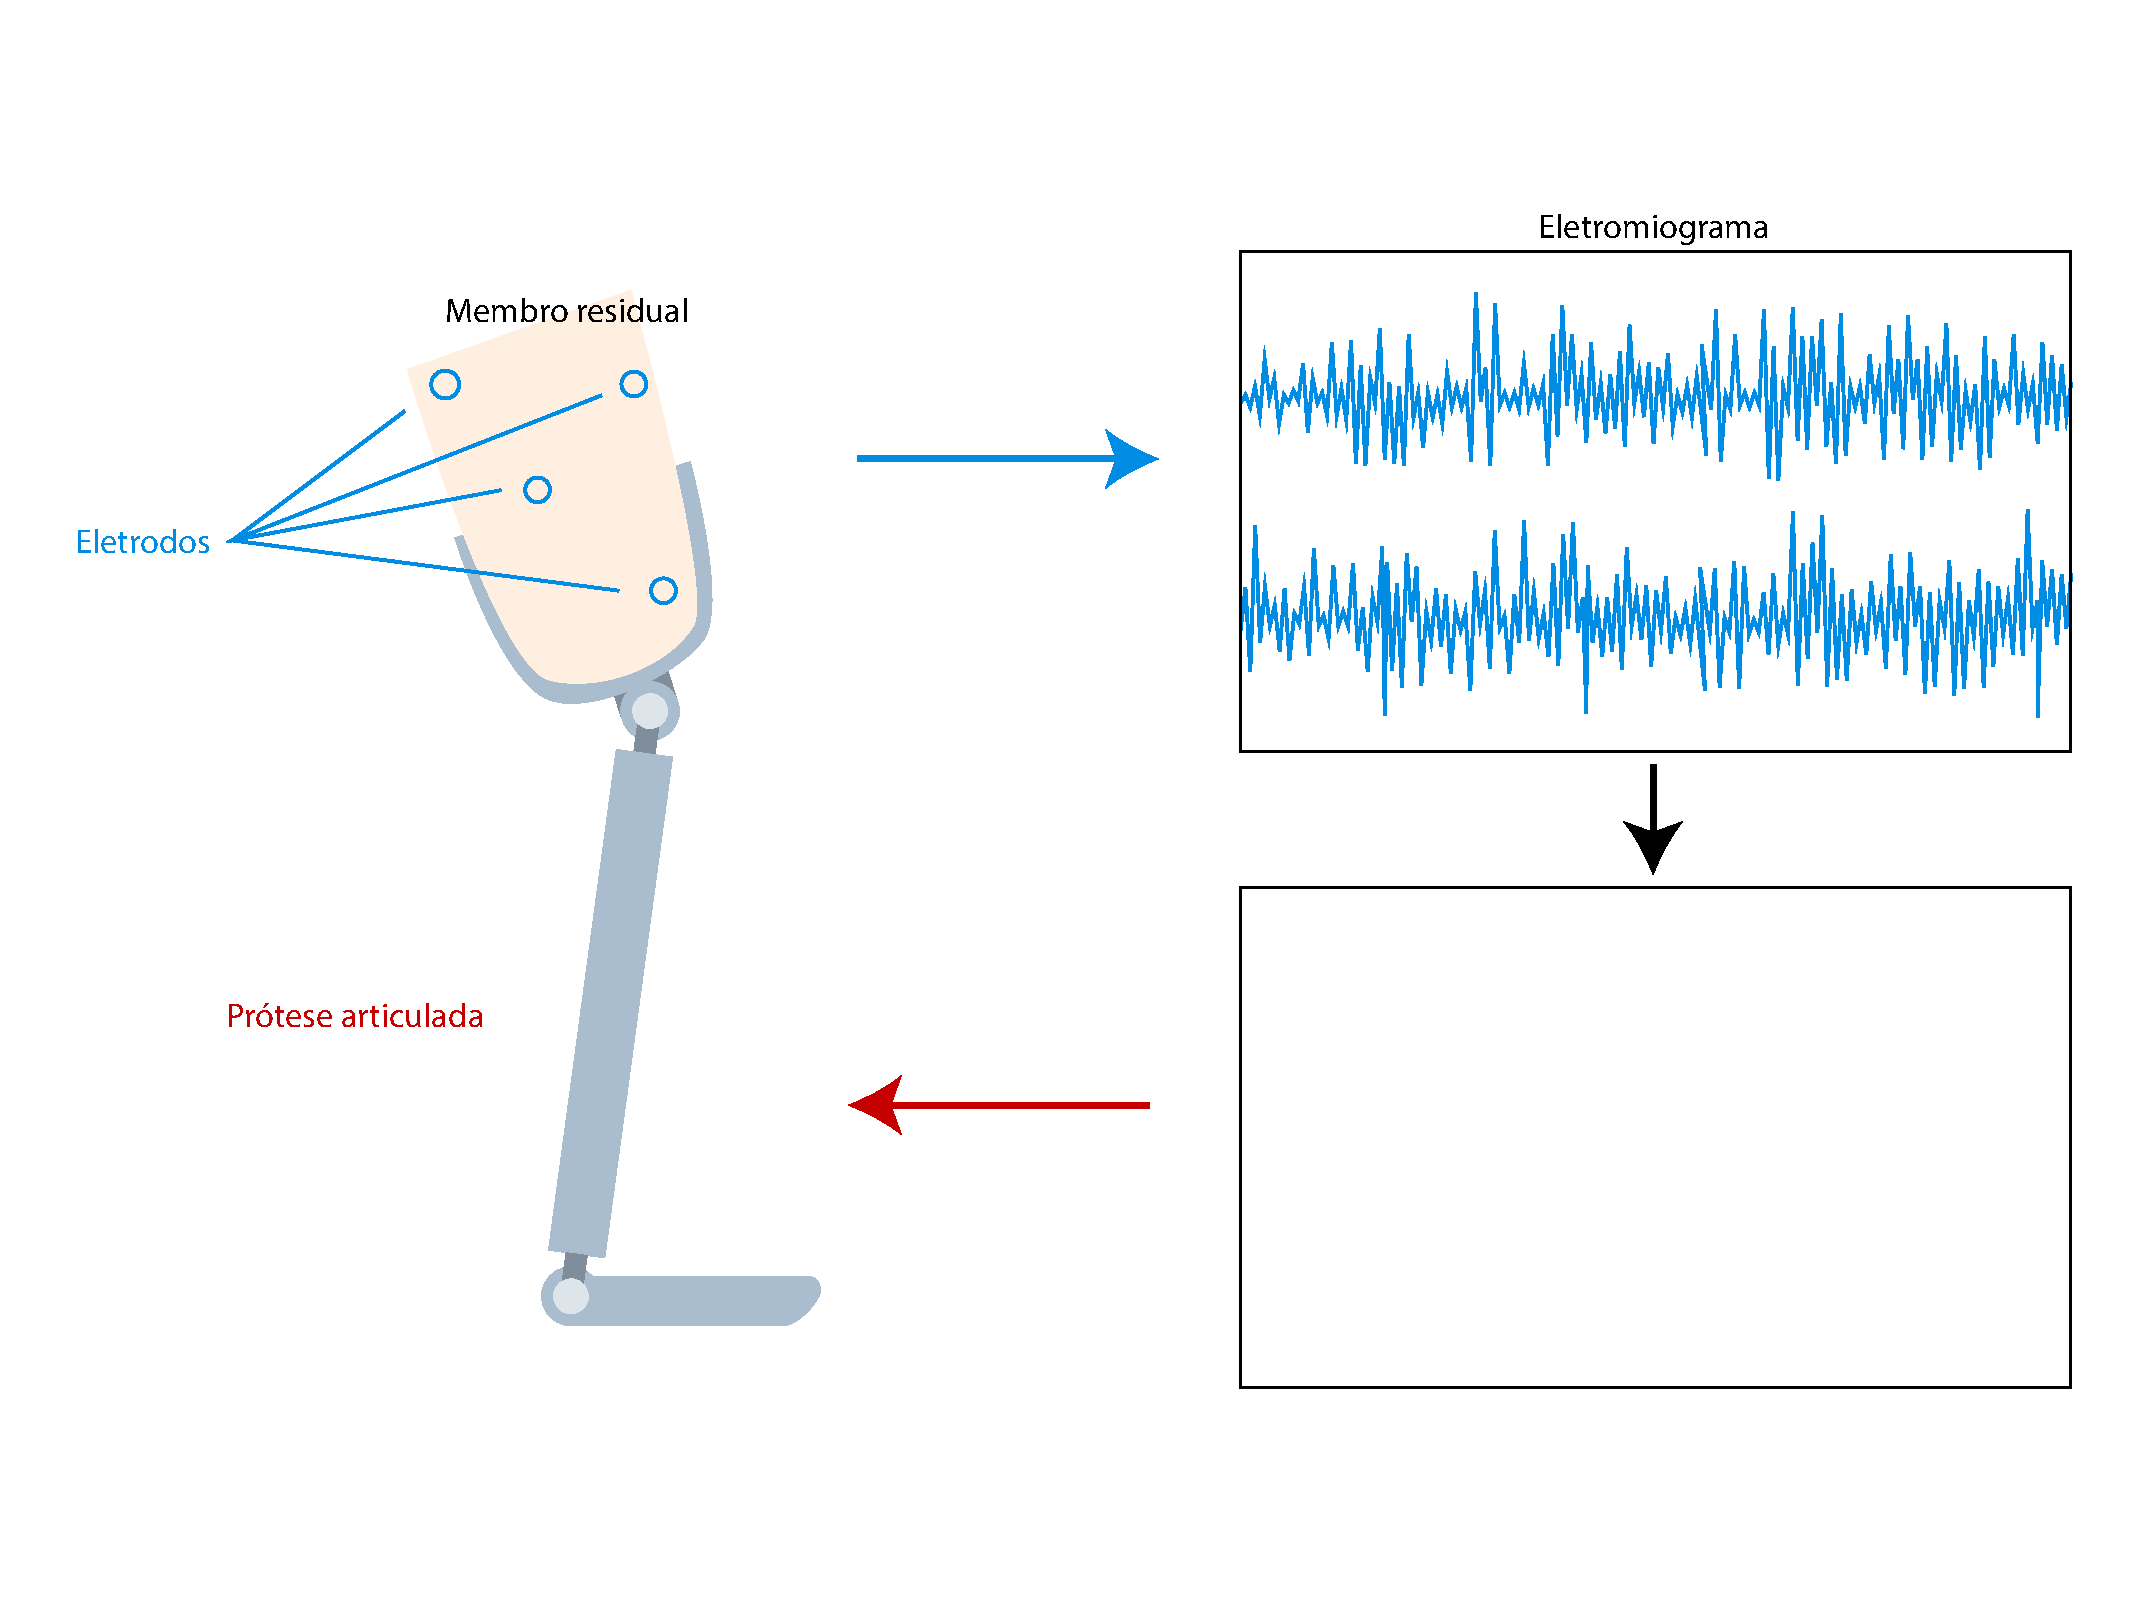
\includegraphics[width=0.6\textwidth]{resources/big_picture}
	\end{center}
	\legend{Fonte: Elaborada pelo autor}
\end{figure}

O sistema computacional que envolve o projeto estará equipado com sensores flex nas articulações dos joelhos além de giroscópios e acelerômetros, que serão usados para capturar as ações do usuário. A figura~\ref{fig:big_picture} ilustra a visão geral do sistema, incluindo o posicionamento dos sensores e o atuador da prótese em si.

Os dados dos sensores serão transmitidos a uma placa de processamento, que se comunicará com o atuador, de forma a adaptar a pisada do usuário de acordo com o ambiente\todo{Como vai ser a fonte de energia da prótese?}. Ou seja, a rigidez da prótese terá diferentes ajustes em caminhadas em planos, subida ou descida de escadas e rampas.

\section{Coleta de dados e classificação}
\todo[inline,color=lightgray]{Coleta de dados dos sensores -- que sensores, que dados. Por que os dados são importantes: usar técnicas pra prever e identificar dados (Seção explicando da coleta, uma seção pra cada tipo de classificação)}

\todo[inline]{\textbf{Nova seção?}}
\todo[inline,color=lightgray]{Geração de movimentos: a partir dos dados coletados. Os atuadores vão tentar identificar os ambientes. Na escada, o motor vai fazer tal coisa, etc. Na rampa, etc.}

\todo[inline]{\textbf{Nova seção?}}
\todo[inline,color=lightgray]{Analisar saúde do caminhar. Se não tá caminhando torto. Gerar estatísticas do uso da prótese. (Os dados estão fazendo a pessoa puxar mais pra uma perna)}